%This is template for your assignment 5 report. Do not change anything in this section if you don't understand it.

\documentclass[paper=a4, fontsize=11pt]{scrartcl} % A4 paper and 11pt font size

\usepackage[T1]{fontenc} % Use 8-bit encoding that has 256 glyphs
\usepackage{fourier} % Use the Adobe Utopia font for the document - comment this line to return to the LaTeX default
\usepackage[english]{babel} % English language/hyphenation
\usepackage{amsmath,amsfonts,amsthm} % Math packages

\usepackage{lipsum} % Used for inserting dummy 'Lorem ipsum' text into the template
\usepackage{caption}
\usepackage{sectsty} % Allows customizing section commands
\allsectionsfont{\centering \normalfont\scshape} % Make all sections centered, the default font and small caps
\usepackage{enumitem}
\usepackage{amssymb}
\usepackage{fancyhdr} % Custom headers and footers
\usepackage{graphicx}
\graphicspath{ {images/} }
\usepackage{tabulary}
\usepackage[left=1in, right=0.5in, top = 0.5in, bottom = 0.5in]{geometry}
\pagestyle{fancyplain} % Makes all pages in the document conform to the custom headers and footers
\fancyhead{} % No page header - if you want one, create it in the same way as the footers below
\fancyfoot[L]{} % Empty left footer
\fancyfoot[C]{} % Empty center footer
\fancyfoot[R]{\thepage} % Page numbering for right footer
\renewcommand{\headrulewidth}{0pt} % Remove header underlines
\renewcommand{\footrulewidth}{0pt} % Remove footer underlines
\setlength{\headheight}{13.6pt} % Customize the height of the header

\numberwithin{equation}{section} % Number equations within sections (i.e. 1.1, 1.2, 2.1, 2.2 instead of 1, 2, 3, 4)
\numberwithin{figure}{section} % Number figures within sections (i.e. 1.1, 1.2, 2.1, 2.2 instead of 1, 2, 3, 4)
\numberwithin{table}{section} % Number tables within sections (i.e. 1.1, 1.2, 2.1, 2.2 instead of 1, 2, 3, 4)

\setlength\parindent{0pt} % Removes all indentation from paragraphs - comment this line for an assignment with lots of text
 
\sectionfont{\bfseries\raggedright}
\subsectionfont{\bfseries\raggedright}

%----------------------------------------------------------------------------------------
%	TITLE SECTION: You can change things below this. Everything is self explanatory.
%----------------------------------------------------------------------------------------

\newcommand{\horrule}[1]{\rule{\linewidth}{#1}} % Create horizontal rule command with 1 argument of height

\title{	
\normalfont \normalsize 
\textsc{Department of Computer Science, LUMS} \\ [25pt] % Your university, school and/or department name(s)
\horrule{0.5pt} \\[0.4cm] % Thin top horizontal rule
\huge Assignment 5: Classification and Neural Networks \\ % The assignment title
\horrule{2pt} \\[0.5cm] % Thick bottom horizontal rule
}

\author{Abdul Maroof (16030010)} % Your name

\date{\normalsize\today} % Today's date or a custom date

\begin{document}

\maketitle % Print the title
%----------------------------------------------------------------------------------------
%	PROBLEM 0
%----------------------------------------------------------------------------------------

\section{Problem 0}

\begin{figure}[h]
\begin{center}
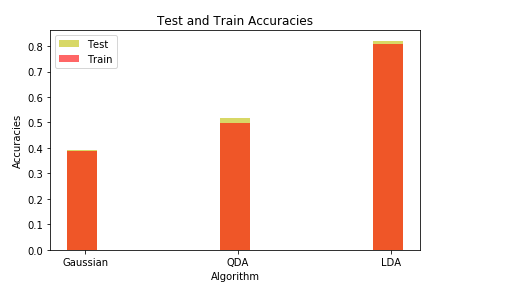
\includegraphics[width=1.4\textwidth]{Question0.png}
\end{center}
\caption{Gaussian vs QDA s LDA}
\label{fig:Question0}
\end{figure}

\subsection{Comment} 
Fisher Linear Discriminant is best as we know that this is a 2 class problem \& we used Gaussian Naive Bayes classifier \& not Multinomial Naive Bayes because the features are continuous.
The best results were shown by Fisher Linear Discriminant as compared to Gaussian Naive Bayes \& Quadratic Discriminant. GNB gave the worst results as Naive Bayes expects discrete values \&  refers to conditional independence of each of the features in the model.

\horrule{0.5pt} \\
\begin{center}
Question 0 ends here.
\horrule{2pt} \\
\end{center}

\pagebreak




%----------------------------------------------------------------------------------------
%	PROBLEM 1
%----------------------------------------------------------------------------------------

\section{Problem 1}

%\subsection{Subsections are made like this (If Required)} 
% Explanation of the outputs goes here
%We have done many things in this course and this is the most difficult one. Still, Figure \ref{fig:demo} shows accuracies over different experiments etc etc. Notice how we used ref to refer the figure by using it's label and latex automatically takes care of numbering.

%New Paragraph can be started with double line space.

%That's how we write subscript $X_i$ and that's how we write super script $X^2$ ...... and that's how we print dollar sign \$. Every mathematical term is required to be encapsulate within dollar sign as we have done with super script and subscript. \% comments out things but adding a forward slash before it prints it in the pdf. Cool. That's all you need to know to make this report. 



\begin{figure}[h]
\begin{center}
\includegraphics[width=1\textwidth]{Question1_Accuracy.png}
\end{center}
\caption{Accuracy Graph of our experiments}
\label{fig:demo}
\end{figure}

\pagebreak


%Question 1 Loss part starts here
\begin{figure}[h]
\begin{center}
\includegraphics[width=1\textwidth]{Question1_Loss.png}
\end{center}
\caption{Loss Graph of our experiments}
\label{fig:demo}
\end{figure}

\subsection{Comment} 
 In most of the cases we see that testing accuracy is slightly better than the training accuracy. Adding  hidden layers decreases our accuracy but increasing the output units with hidden layers gives better results as compare to adding layer with less output units.

\horrule{0.5pt} \\
\begin{center}
Question 1 ends here.
\horrule{2pt} \\
\end{center}
\pagebreak


%----------------------------------------------------------------------------------------
%	PROBLEM 2
%----------------------------------------------------------------------------------------

\section{Problem 2}

All the functions are implemented and could be found in $functions$ folder. We have used the fields of downloaded data that were most likely to help us detecting duplicate entries. Two fields that are selected for this purpose are $titles$ \& $description$. However other fields can be added but it did'nt help much.

We have set the random seed generation to 100 for reproducibility of the results. Following table summarizes the results obtained with accuracy more than 80\%.

\begin{center}
\captionof{table}{Accuracy Graph of our experiments}
\begin{tabulary}{1\textwidth}{|L|L|L|}


\hline
\hline
- & FeedForward Network & Convolutional Network  \\ 
\hline
\hline
Train Accuracy & 0.8 & 0.9    \\
\hline
Validation Accuracy & 0.9 & 0.95 \\
\hline
Test Accuracy & 0.25 & 0.55  \\
\hline
\end{tabulary}
\end{center}

\begin{figure}[h]
\begin{center}
\includegraphics[width=1\textwidth]{Question2_Accuracy.png}
\end{center}
\caption{Accuracy Graph of our experiments}
\label{fig:demo}
\end{figure}


\pagebreak
%Problem 2 Loss graph is under


\begin{figure}[h]
\begin{center}
\includegraphics[width=1\textwidth]{Question2_Loss.png}
\end{center}
\caption{Loss Graph of our experiments}
\label{fig:demo}
\end{figure}

\subsection{Comment} 
Combination of Relu(hidden) and Softmax(output) with Mean Square Error gives better results. as  we have also done one hot encoding in softmax as it is used for continuous values. and also in this case we have used categorical cross entropy as it's for more then 2 classes we have use softmaax


\horrule{0.5pt} \\
\begin{center}
Question 2 ends here.
\horrule{2pt} \\
\end{center}


\pagebreak


%----------------------------------------------------------------------------------------
%	PROBLEM 3
%----------------------------------------------------------------------------------------

\section{Problem 3}
Everything Regrading Problem 3 goes here.

\begin{figure}[h]
\begin{center}
\includegraphics[width=1\textwidth]{Question3_Accuracy.png}
\end{center}
\caption{Accuracy Graph of our experiments}
\label{fig:demo}
\end{figure}

% %Problem 3 Loss graph is under


\pagebreak
\begin{figure}[h]
\begin{center}
\includegraphics[width=1\textwidth]{Question3_Loss.png}
\end{center}
\caption{Loss Graph of our experiments}
\label{fig:demo}
\end{figure}

\subsection{Comment} 
 The accuracy \& loss coverged eventually for all variaites of momentun \& learning rate so this isn't has much affect on our model
\horrule{0.5pt} \\
\begin{center}
Question 3 ends here.
\horrule{2pt} \\
\end{center}

%----------------------------------------------------------------------------------------
%	PROBLEM 4
%----------------------------------------------------------------------------------------

\pagebreak
\section{Problem 4}
\begin{figure}[h]
\begin{center}
\includegraphics[width=1\textwidth]{Question4_Accuracy.png}
\end{center}
\caption{Accuracy Graph of our experiments}
\label{fig:demo}
\end{figure}

\pagebreak

% %Problem 3 Loss graph is under
\begin{figure}[h]
\begin{center}
\includegraphics[width=1\textwidth]{Question4_Loss.png}
\end{center}
\caption{Loss Graph of our experiments}
\label{fig:demo}
\end{figure}

\subsection{Comment} 
Results are better in case of SGD\& rmsprop. Results are also good for adam \& nadam as we can see in figure 5.1 that they are approx. converging after some time.

\horrule{0.5pt} \\
\begin{center}
Question 4 ends here.
\horrule{2pt} \\
\end{center}
\pagebreak
 

%----------------------------------------------------------------------------------------
%	PROBLEM 5
%----------------------------------------------------------------------------------------

\section{Problem 5}


\subsection{Comments} 
Convolution layer learns about the features.

Neural Networks has to learn only the extracted features when we add convolutional  layer \& when we dont then it would have to learn the whole model.
Max pooling is necessary to add after convolution layer so that we can have a bit of distortion to aviod linearity.

Adding more layers in case when you have a lot of data \& diversified data then then it's a smart and good choice and adding layers when you have very limited data may not perform that well.

 Deep learning is better to get classifications of a diversified data. It is basically combination of many nerual network layers like convolution and fully connected layers and some other layers like max pool etc. Deep Learning refers to Neural Network models with generally more than 2 or 3 hidden layers. It's a large multi layered Neural Network model that requires lots of data.

\horrule{0.5pt} \\
\begin{center}
Question 5 ends here.
\horrule{2pt} \\
\end{center}
\pagebreak


%----------------------------------------------------------------------------------------

\end{document}